% Behavior tree of The Archivist, Vagrancy (data/pilots.json, "archivist").
% Standalone: compiles on its own in Overleaf with pdflatex.
\documentclass[tikz,border=4pt]{standalone}
\usetikzlibrary{arrows.meta,shapes.geometric,positioning,calc}

% --- Colors: the deck's palette --------------------------------------------
\definecolor{paper}{HTML}{FDFDFC}   % background
\definecolor{ink}{HTML}{1B2430}     % text and edges
\definecolor{muted}{HTML}{6B7680}   % legend and notes
\definecolor{cond}{HTML}{2F4BA0}    % condition leaves
\definecolor{act}{HTML}{2A6B4A}     % action leaves
\definecolor{intr}{HTML}{8B2E2E}    % rules that interrupt a running move

% --- Layout, in centimetres --------------------------------------------------
\newcommand{\NumRules}{3}         % rules with a condition, left to right in priority order
\newcommand{\ColGap}{4.2}           % horizontal distance between rule columns
\newcommand{\BoxW}{3.7cm}           % width of every leaf box
\newcommand{\BusY}{-1.2}            % height of the bar the root's children hang from
\newcommand{\SeqY}{-2.2}            % height of the sequence nodes
\newcommand{\CondY}{-4.4}           % height of the condition leaves
\newcommand{\ActY}{-7.0}            % height of the action leaves
\newcommand{\Reaction}{6}     % reaction time, ticks (data/pilots.json)
\newcommand{\ReactionMs}{100}      % the same, milliseconds, at 60 ticks a second

\begin{document}
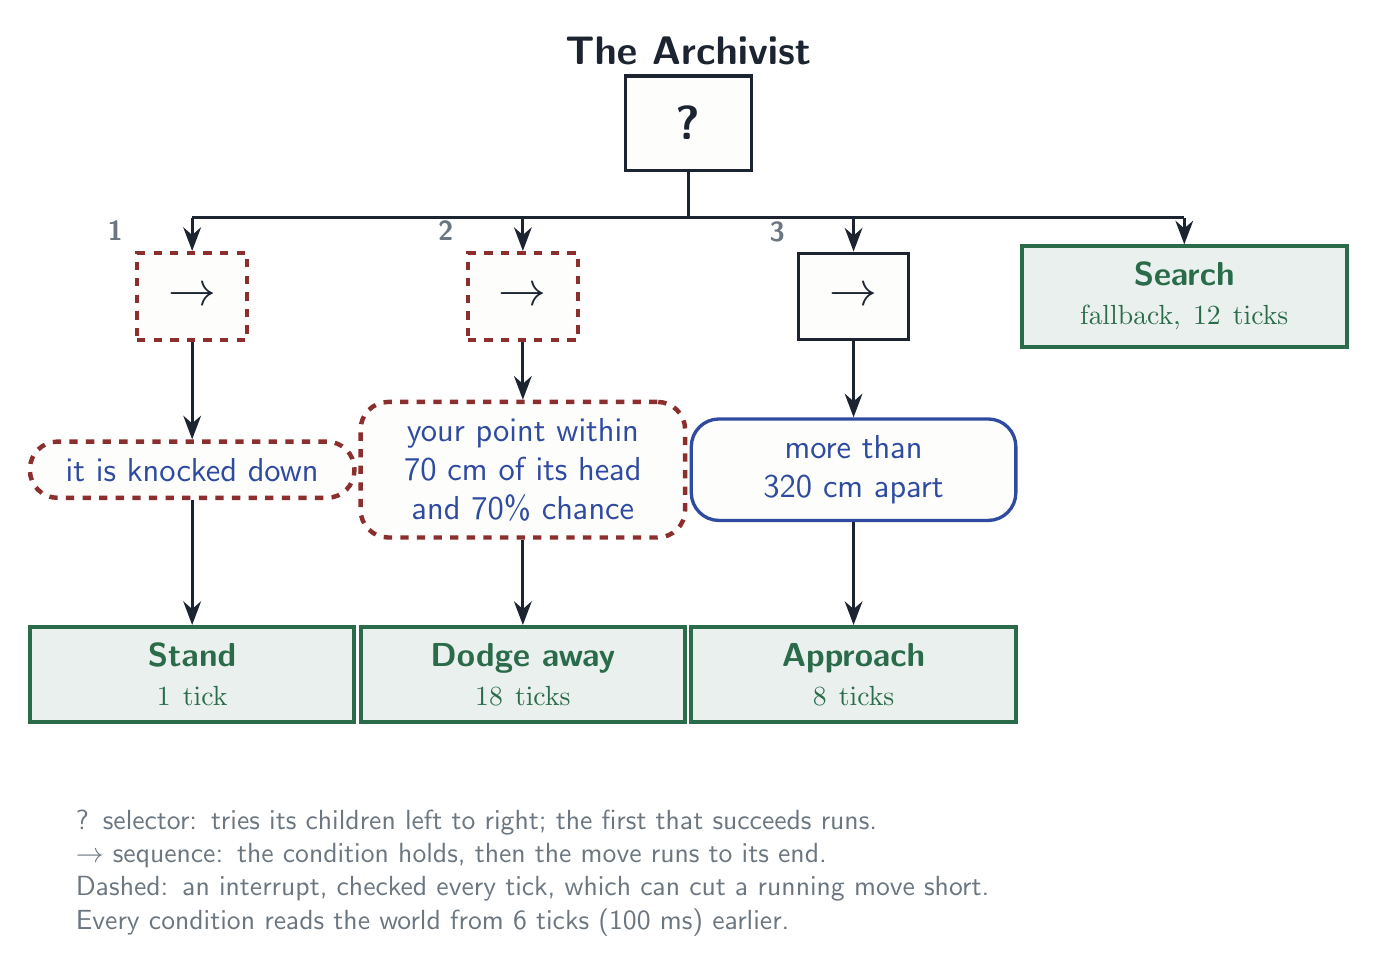
\begin{tikzpicture}[
    font=\sffamily\large, ink,
    edge/.style={-{Stealth[length=3mm]}, line width=1pt, draw=ink},
    selector/.style={draw=ink, line width=1.2pt, fill=paper, minimum width=1.6cm, minimum height=1.2cm, font=\sffamily\bfseries\LARGE},
    sequence/.style={draw=ink, line width=1.2pt, fill=paper, minimum width=1.4cm, minimum height=1.1cm, font=\sffamily\bfseries\LARGE},
    intr0/.style={},
    intr1/.style={draw=intr, dashed, line width=1.6pt},
    condition/.style={draw=cond, line width=1.2pt, rounded corners=10pt, fill=paper, text width=\BoxW, align=center, inner sep=6pt, text=cond},
    action/.style={draw=act, line width=1.4pt, fill=act!10, text width=\BoxW, align=center, inner sep=6pt, text=act, font=\sffamily\large\bfseries},
  ]

% --- Root: a selector over the rules, highest priority on the left ----------
\node[selector] (root) at ({\NumRules*\ColGap/2}, 0) {?};
\node[anchor=south, font=\sffamily\bfseries\Large] at (root.north) {The Archivist};

% --- One sequence per rule: its condition, then its move ---------------------
\foreach \i/\cond/\act/\ticks/\intr in {1/{it is knocked down}/{Stand}/{1 tick}/1, 2/{your point within 70 cm of its head \\ and 70\% chance}/{Dodge away}/{18 ticks}/1, 3/{more than 320 cm apart}/{Approach}/{8 ticks}/0} {
  \pgfmathsetmacro{\x}{(\i-1)*\ColGap}
  \node[sequence, intr\intr] (s\i) at (\x, \SeqY) {$\rightarrow$};
  \node[condition, intr\intr] (c\i) at (\x, \CondY) {\cond};
  \node[action] (a\i) at (\x, \ActY) {\act \\ {\normalfont\normalsize \ticks}};
  \draw[edge] (\x, \BusY) -- (s\i.north);
  \draw[edge] (s\i.south) -- (c\i.north);
  \draw[edge] (c\i.south) -- (a\i.north);
  \node[font=\sffamily\bfseries\normalsize, text=muted] at ($(s\i.north west)+(-0.25,0.25)$) {\i};
}

% --- The fallback: the move when no rule's condition holds ------------------
\pgfmathsetmacro{\fx}{\NumRules*\ColGap}
\node[action] (fallback) at (\fx, \SeqY) {Search \\ {\normalfont\normalsize fallback, 12 ticks}};
\draw[edge] (\fx, \BusY) -- (fallback.north);

% --- The bar: the root drops to it, and every child hangs from it ------------
\draw[line width=1pt, draw=ink] (root.south) -- ({\NumRules*\ColGap/2}, \BusY);
\draw[line width=1pt, draw=ink] (0, \BusY) -- (\fx, \BusY);

% --- Annotations -------------------------------------------------------------
\node[anchor=north west, text=muted, font=\sffamily\normalsize, align=left, text width={(\NumRules*\ColGap+3.2)*1cm}] at (-1.6, -8.6)
  {? selector: tries its children left to right; the first that succeeds runs.\\
    $\rightarrow$ sequence: the condition holds, then the move runs to its end.\\
    Dashed: an interrupt, checked every tick, which can cut a running move short.\\
    Every condition reads the world from \Reaction{} ticks (\ReactionMs{} ms) earlier.};

\end{tikzpicture}
\end{document}

% --- Self-check ----------------------------------------------------------------
% Rule order: the \foreach list is data/pilots.json's rules for "archivist", in order; the
%   selector reads them left to right, so left is higher priority (root at the top).
% Interrupts: rules with "interrupt": true carry intr1 (dashed, brick) on their sequence
%   and condition nodes; the others carry intr0.
% Fallback: the rule with no condition ("search") hangs directly off the root, last.
% Durations: each move's length in ticks comes from Tree::play in crates/pilot/src/lib.rs
%   ("1 tick", otherwise "N ticks").
% Edges: the root drops to one bar at \BusY and every child hangs from it, so no edge
%   crosses a node.
% Reaction: \Reaction is "reaction_ticks" (6); \ReactionMs is ceil(6 x 1000 / 60).
